\documentclass{article}
\usepackage{../../Self_Style}

\title{Phys 115A HW 4}
\author{Zih-Yu Hsieh}
\date{\today}

\begin{document}
\maketitle

\section*{1}
\begin{ques}\label{q1}
Euler Equivalence (Griffiths 2.17)

Show that $A e^{ikx} + B e^{-ikx}$ and $C \cos kx + D \sin kx$ are equivalent ways of writing the same function of $x$, and determine the constants $C$ and $D$ in terms of $A$ and $B$ and vice versa. In quantum mechanics, when $V = 0$, the exponentials represent traveling waves, and are most convenient in discussing the free particle, whereas sines and cosines correspond to standing waves, which arise naturally in the case of the infinite square well.
\end{ques}

\begin{proof}
    Given Euler's formula $e^{it}=\cos(t)+i\sin(t)$, then the first expression can be rewrite as follow:
    \begin{align}
        Ae^{ikx}+Be^{-ikx}=A(\cos(kx)+i\sin(kx))+B(\cos(-kx)+i\sin(-kx)) = (A+B)\cos(kx)+i(A-B)\sin(kx)
    \end{align}
    Hence, to express $Ae^{ikx}+Be^{-ikx}=C\cos(kx)+D\sin(kx)$, one has $C=A+B$ and $D=i(A-B)$.

    Equivalently, since $C=A+B$ and $-iD=A-B$, then $A=\frac{C-iD}{2}$ and $B=\frac{C+iD}{2}$.
\end{proof}

\hfil

\section*{2}
\begin{ques}\label{q2}
Free Currents (Griffiths 2.18)

Find the probability current, $J$, for the free particle wave function in Eq. 2.95, $\Psi_k(x, t) = A e^{i(kx - \hbar k^2 t / 2m)}$. Which direction does the probability current flow?
\end{ques}

\begin{proof}
    Given the probability current $J(x,t)=-\frac{i\hbar}{2m}\left(\Psi^*\frac{\partial\Psi}{\partial x}-\Psi\frac{\partial\Psi^*}{\partial x}\right)$, given $\Psi_k(x,t)=Ae^{i(kx-\hbar k^2t/2m)}$, then $\frac{\partial\Psi_k}{\partial x}=ikAe^{i(kx-\hbar k^2t/2m)} = ik\Psi_k$. Hence, the probability current is as follow:
    \begin{align}
        J(x,t) = -\frac{i\hbar}{2m}\left(\Psi_k^* \cdot ik\Psi_k - \Psi_k \cdot (-ik\Psi_k^*)\right) = -\frac{i\hbar}{2m}\cdot 2ik|\Psi_k|^2 = \frac{k\hbar}{m}
    \end{align}
    This indicates that the direction of the probability current is flowing in the positive direction, which fits with the fact that $\Psi_k(x,t)$ represents a wave traversing in the positive $x$ direction.
\end{proof}

\newpage

\section*{3}
\begin{ques}\label{q3}
Born Free (Modified Griffiths 2.20)

Consider a free particle whose state at time $t = 0$ is given by $\Psi(x, 0) = A e^{-a^2 |x|}$ for real constants $A, a$.

\begin{enumerate}
    \item Normalize $\Psi(x, 0)$.
    \item Find $\phi(k)$ for this wavefunction.  
    \item Construct $\Psi(x, t)$; you can leave it in the form of an integral. 
    \item What is the shape of $\Psi(x, 0)$ and $\phi(k)$, respectively, when $a \gg 1$? When $a \ll 1$?
\end{enumerate}
\end{ques}

\begin{proof}
    Given $\Psi(x,0)=Ae^{-a^2|x|}$, then it's of the following form:
    \begin{align}
        \Psi(x,0)=\begin{cases}
            Ae^{-a^2x} & x\geq 0\\
            Ae^{a^2x} & x<0
        \end{cases}
    \end{align}

    \begin{itemize}
        \item[1.] To normalize $\Psi(x,0)$, we want $\int_{-\infty}^{\infty}|\Psi|^2dx=1$, which can be expressed as follow:
        \begin{align}
            1&=\int_{-\infty}^{\infty}|\Psi|^2 dx = \int_{-\infty}^{0}A^2e^{2a^2x}dx + \int_{0}^{\infty}A^2e^{-2a^2x}dx\\
            &= \int_{-\infty}^{0}A^2e^{2a^2x}dx-\int_{0}^{-\infty}A^2e^{2a^2u}(-1)du\\
            &= 2\int_{-\infty}^{0}A^2e^{2a^2x}dx = \frac{2A^2}{2a^2}e^{2a^2x}\bigg|_{-\infty}^{0} = \frac{A^2}{a^2}
        \end{align}
        Hence, $\frac{A^2}{a^2}=1, A^2=a^2$, which implies that $A=\pm a$. For simplicity, one can choose $A=a$, hence $\Psi(x,0)=ae^{-a^2|x|}$.

        \hfil

        \item[2.] To express the Fourier Transform, ew have $\Psi(x,0)=\frac{1}{\sqrt{2\pi}}\int_{-\infty}^{\infty}\phi(k)e^{ikx}dk$, which $\phi(k)$ can be expressed as follow using Inverse Fourier Transform:
        \begin{align}
            \phi(k)&=\frac{1}{\sqrt{2\pi}}\int_{-\infty}^{\infty}\Psi(x,0)e^{-ikx}dx = \frac{1}{\sqrt{2\pi}}\left(\int_{-\infty}^{0}ae^{a^2x}e^{-ikx}dx+\int_{0}^{\infty}ae^{-a^2x}e^{-ikx}dx\right)\\
            &= \frac{1}{\sqrt{2\pi}}\left(\frac{a}{a^2-ik}e^{a^2x}e^{-ikx}\bigg|_{-\infty}^{0}+\frac{a}{-a^2-ik}e^{-a^2x}e^{-ikx}\bigg|_{0}^{\infty}\right)\\
            &= \frac{1}{\sqrt{2\pi}}\left(\frac{a}{a^2-ik}+\frac{a}{a^2+ik}\right) = \frac{a}{\sqrt{2\pi}}\frac{(a^2+ik)+(a^2-ik)}{a^4+k^2} = \frac{2a^3}{\sqrt{2\pi}(a^4+k^2)}    
        \end{align}

        \hfil

        \item[3.] In integral expression, the full wave function is as follow:
        \begin{align}
            \Psi(x,t) = \frac{1}{\sqrt{2\pi}}\int_{-\infty}^{\infty}\phi(k)e^{i(kx-\hbar k^2t/2m)}dk =\int_{-\infty}^{\infty}\frac{a^3}{\pi(a^4+k^2)}e^{i(kx-\hbar k^2t/2m)}dk
        \end{align}

        \hfil

        \item[4.] When $a\gg 1$, the following are the two figures of $\Psi(x,0)$ and $\phi(k)$ respectively:
        \begin{figure}[h!]
            \centering
            % First subfigure
            \begin{subfigure}[b]{0.9\textwidth}
                \centering
                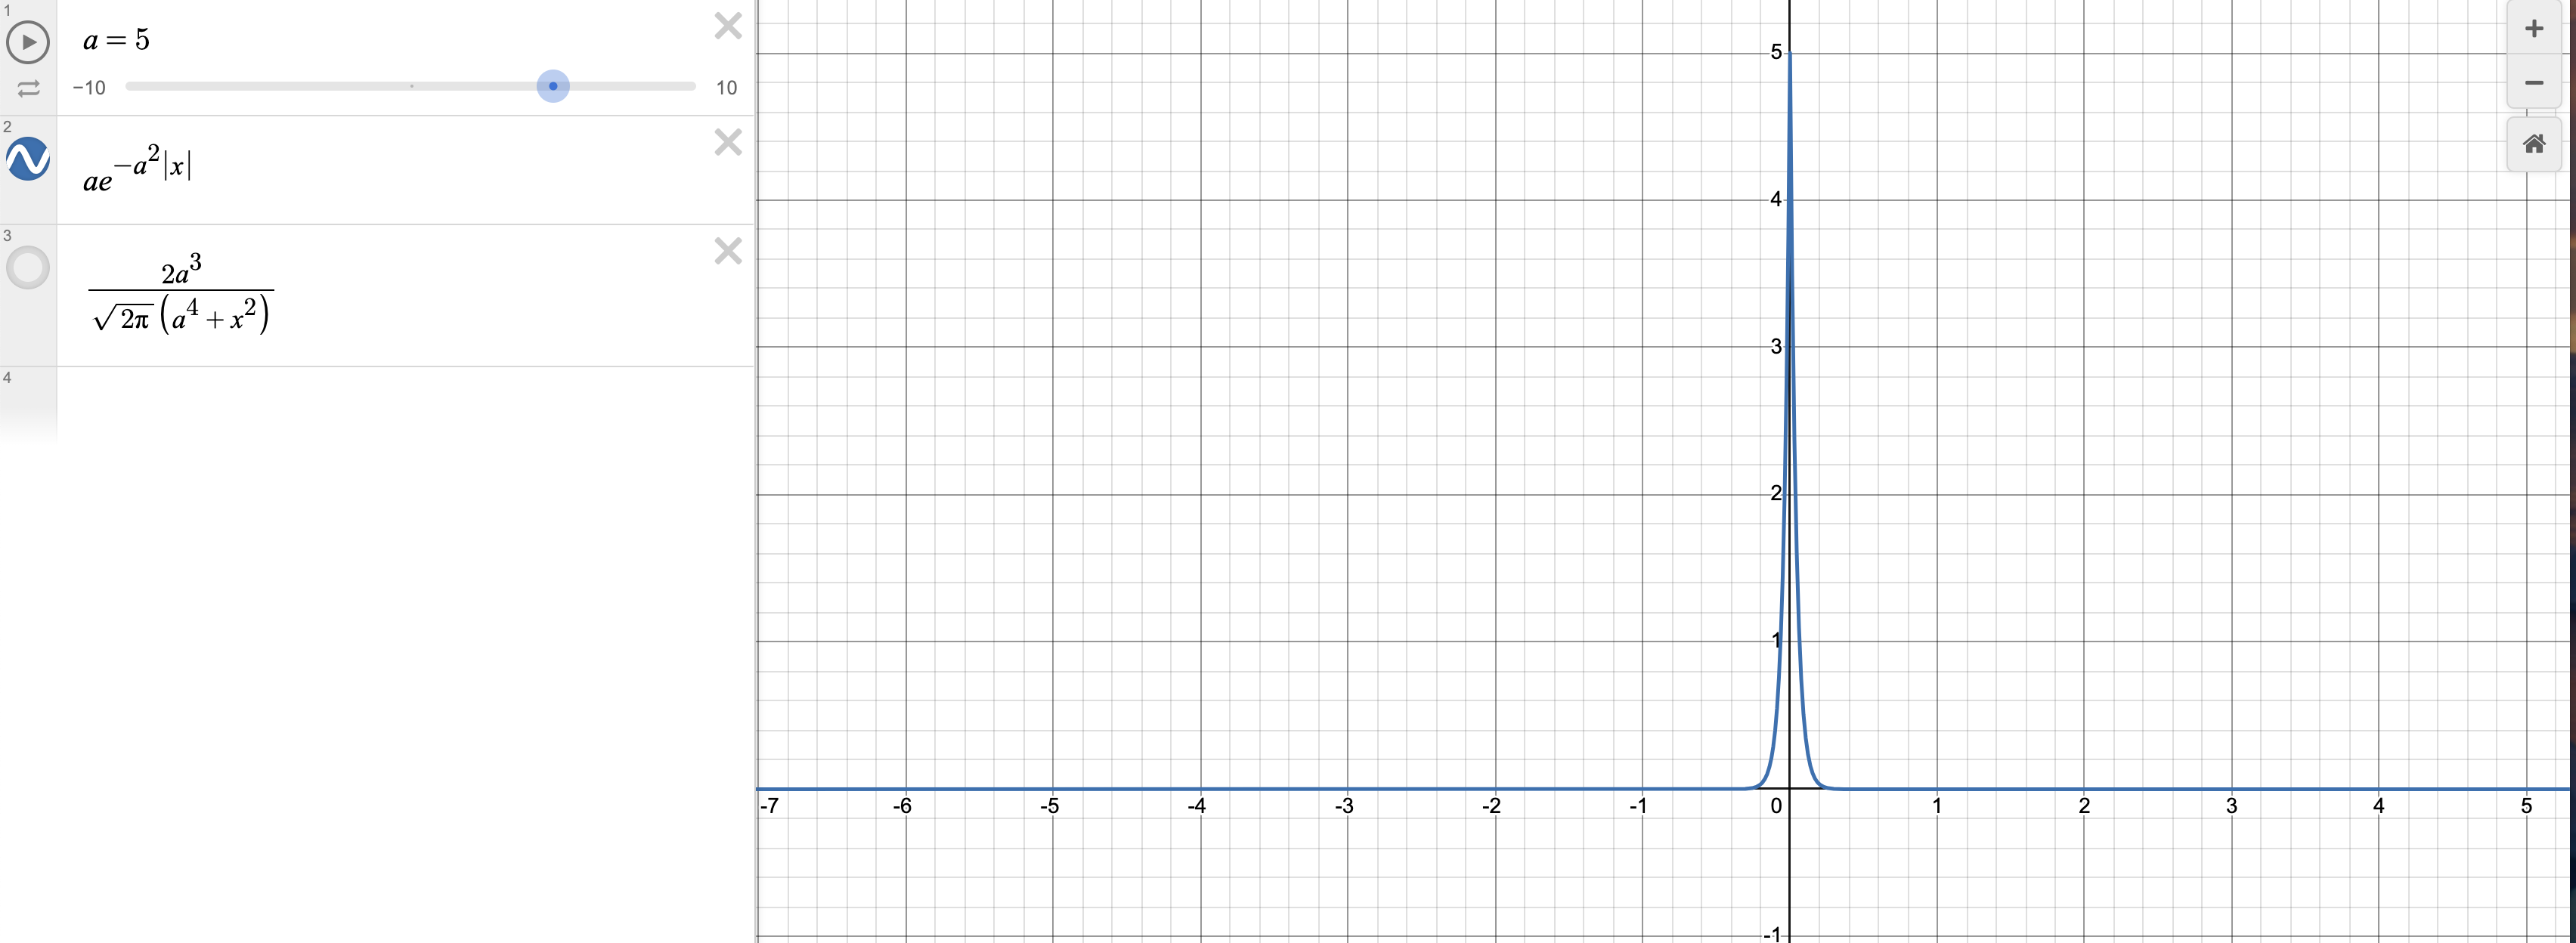
\includegraphics[width=\textwidth]{x1.png}
                \caption{Graph of $\Psi(x,0)$, $a\gg 1$}
                \label{fig:x1}
            \end{subfigure}

            \hfill

            % Second subfigure
            \begin{subfigure}[b]{0.9\textwidth}
                \centering
                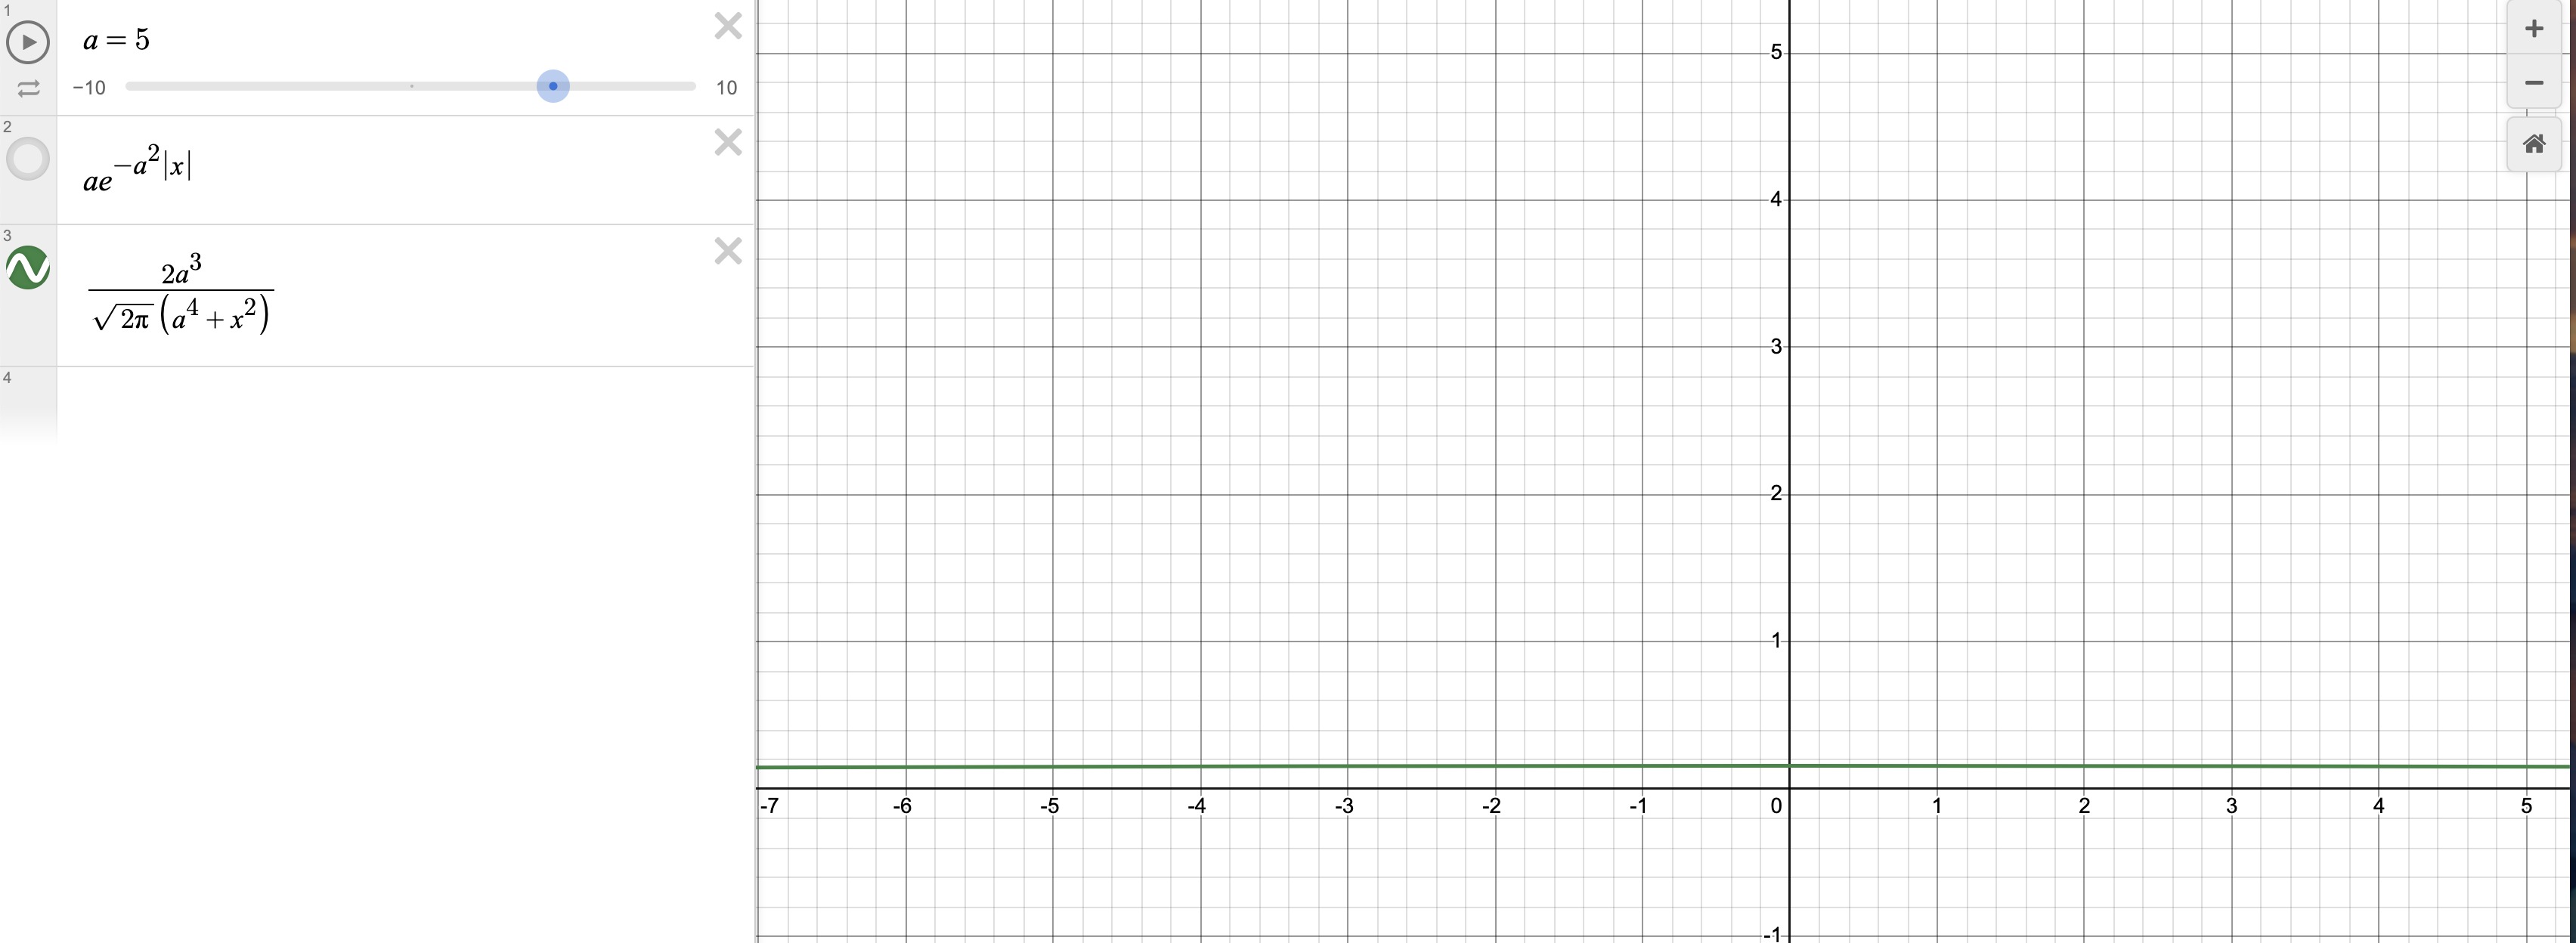
\includegraphics[width=\textwidth]{p1.png}
                \caption{Graph of $\phi(k)$, $a\gg 1$}
                \label{fig:p1}
            \end{subfigure}
            \label{fig:xp1}
        \end{figure}

        \newpage

        Which, one can observe a high and narrow spike in $\Psi(x,0)$, while $\phi(k)$ is low and spread out.

        \hfil

        On the other hand, when $a\ll 1$, the following are the two figures of $\Psi(x,0)$ and $\phi(k)$ respectively:
        \begin{figure}[h!]
            \centering
            % First subfigure
            \begin{subfigure}[b]{0.9\textwidth}
                \centering
                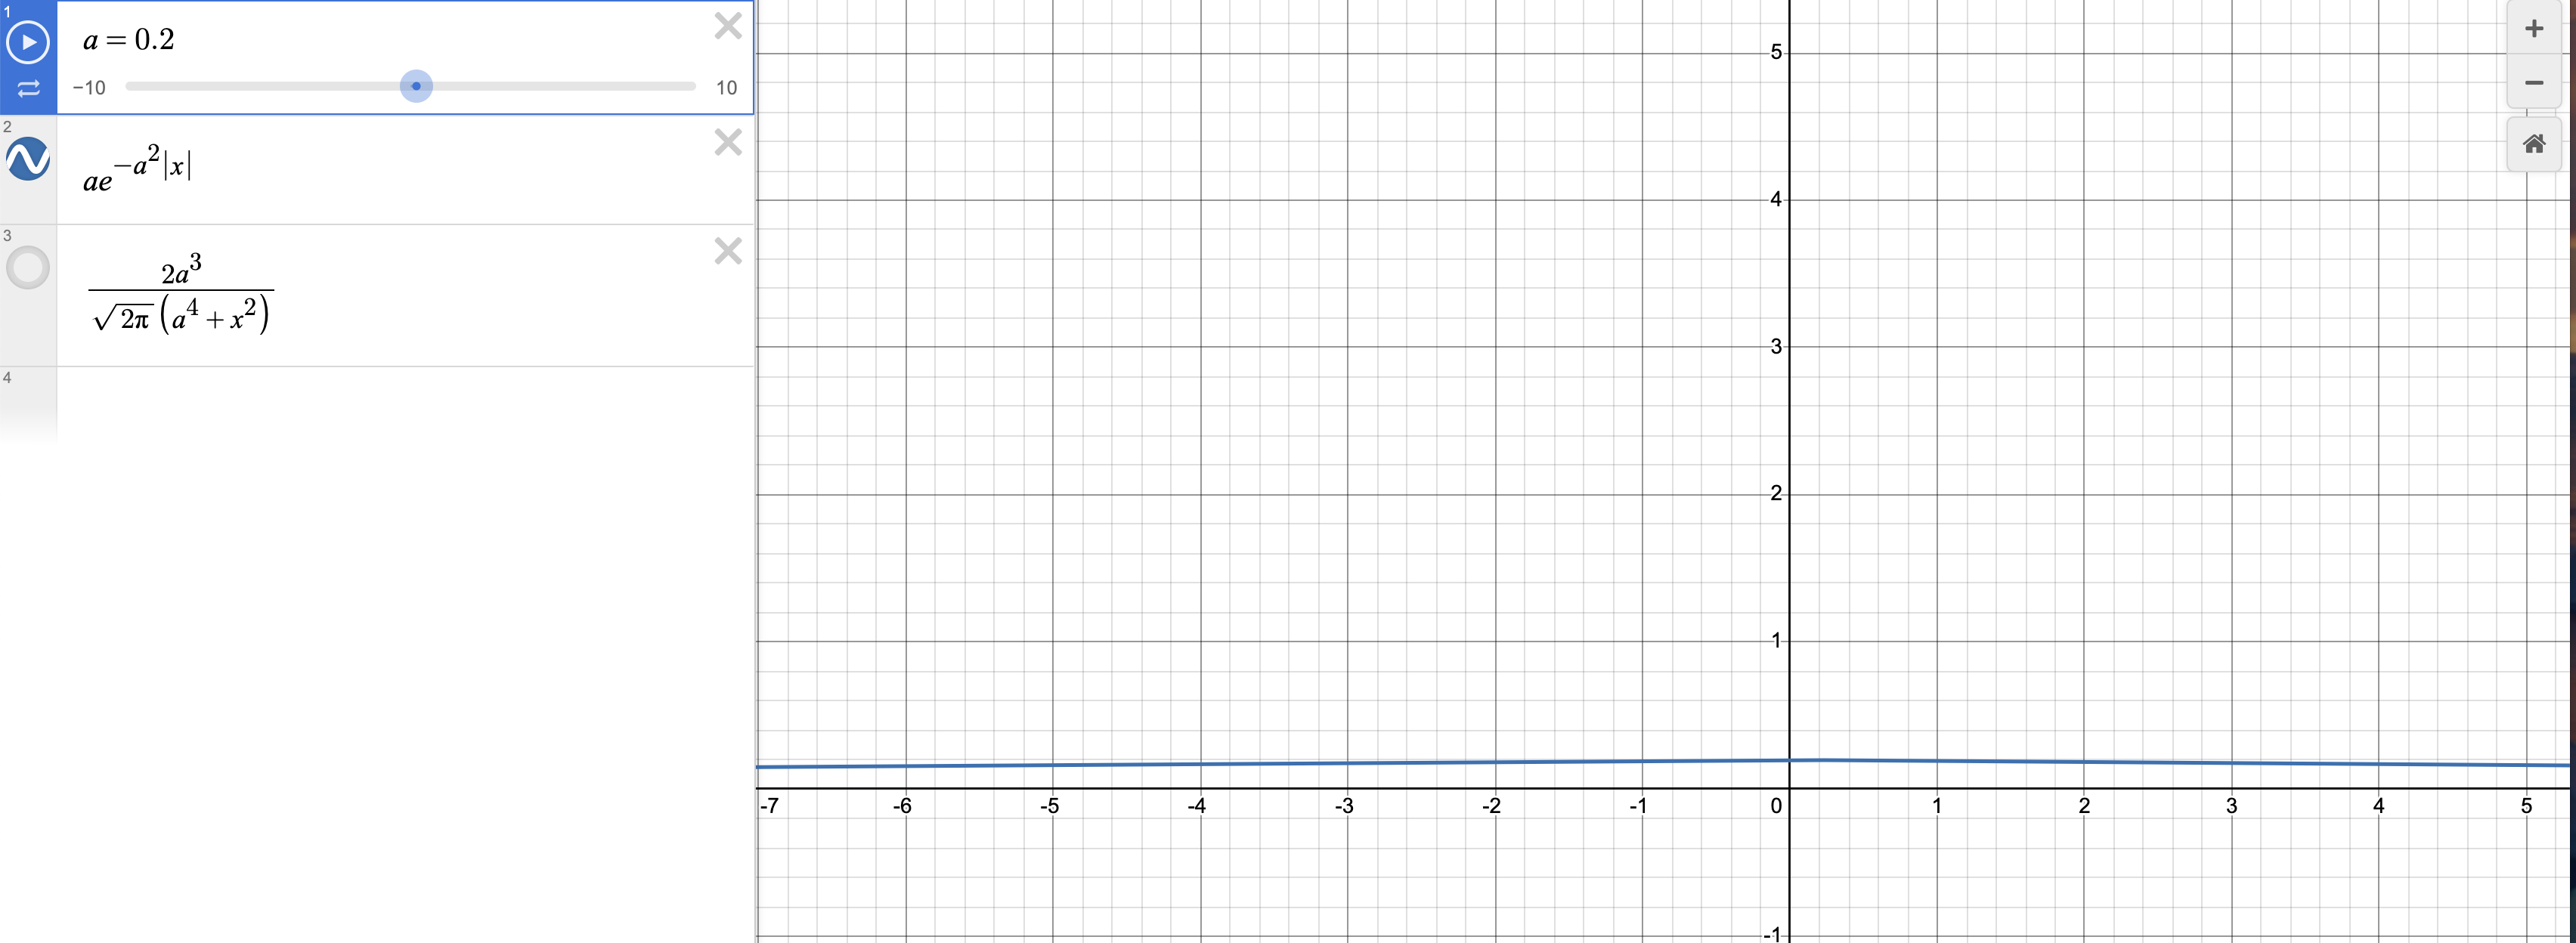
\includegraphics[width=\textwidth]{x2.png}
                \caption{Graph of $\Psi(x,0)$, $a\ll 1$}
                \label{fig:x2}
            \end{subfigure}

            \hfill

            % Second subfigure
            \begin{subfigure}[b]{0.9\textwidth}
                \centering
                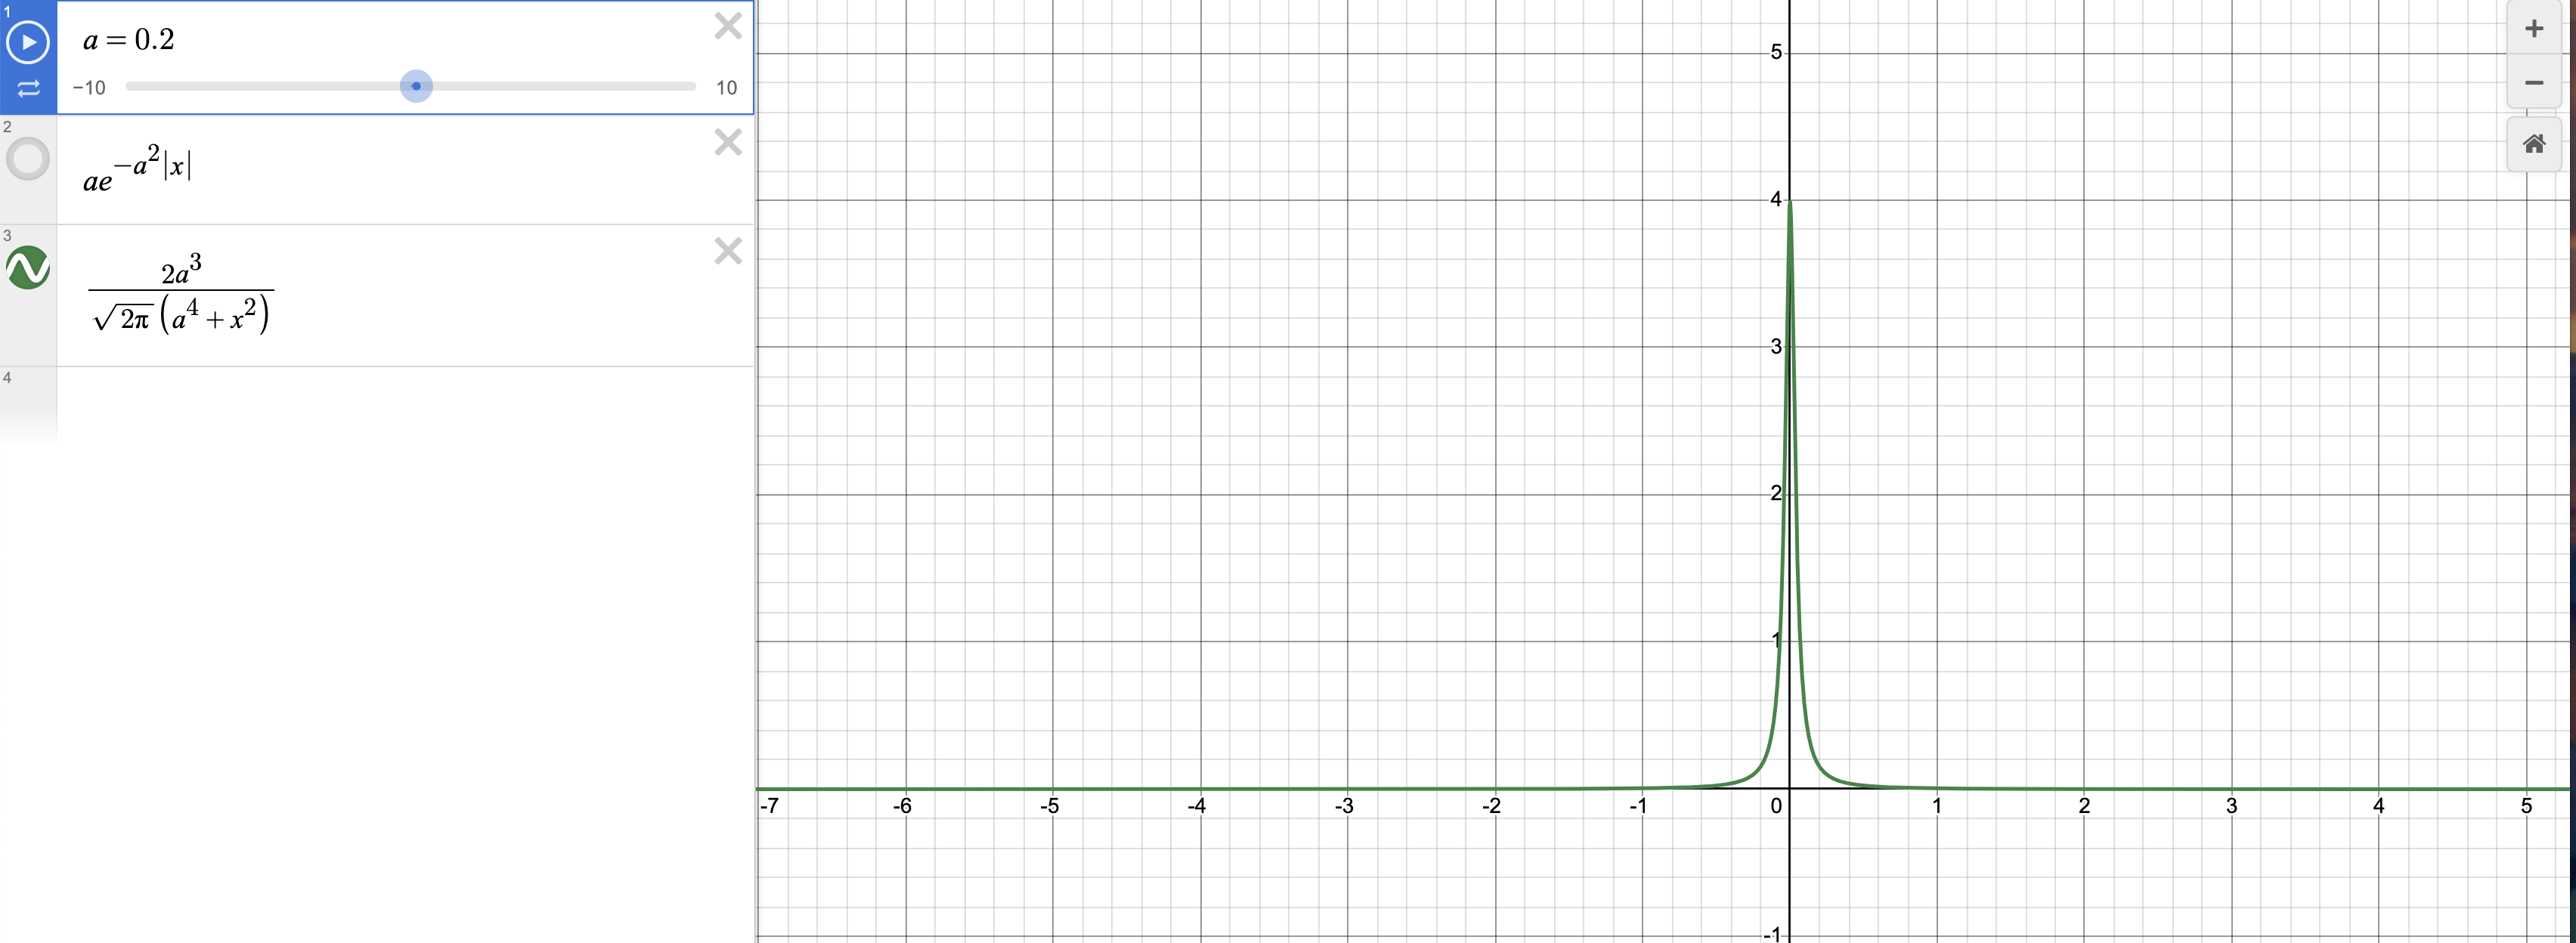
\includegraphics[width=\textwidth]{p2.png}
                \caption{Graph of $\phi(k)$, $a\ll 1$}
                \label{fig:p2}
            \end{subfigure}
            \label{fig:xp2}
        \end{figure}

        \newpage

        Now, the graphs are in reverse, where $\Psi(x,0)$ is low and spread out, while $\phi(k)$ is with a high and narrow spike.
    \end{itemize}
\end{proof}

\newpage

\section*{4 (ND)}
\begin{ques}\label{q4}
Rockin’ in the Free World (Modified Griffiths 2.21)

Consider a free particle whose state at time $t = 0$ is given by a gaussian wave packet, $\Psi(x, 0) = A e^{-a^2 x^2}$ for real constants $A, a$.

\begin{enumerate}
\item Normalize $\Psi(x, 0)$, i.e., find $A$.  
\item Find $\Psi(x, t)$. You can do the integral by completing the square in the exponent to get it into the form of a gaussian: let $y = \sqrt{a}[x + (b/2a)]$, and note that $(a x^2 + b x) = y^2 - (b^2 / 4a)$.  
\item Compute the probability density $|\Psi(x, t)|^2$, expressing your answer in terms of $w \equiv a \sqrt{1 + (2\hbar a^2 t / m)^2}$. Sketch the probability density as a function of $x$ for $t = 0$, and again for some large $t$. What’s happening to $|\Psi|^2$ as time evolves?  
\item Find the usual suspects, $\langle x \rangle, \langle p \rangle, \langle x^2 \rangle, \langle p^2 \rangle, \sigma_x, \sigma_p$. Although tedious, they ultimately have relatively compact forms: partial answer $\langle p^2 \rangle = a^2 \hbar^2$.  
\item Verify that the uncertainty principle holds. At what $t$ do we come closest to saturating the uncertainty principle? Why?
\end{enumerate}
\end{ques}

\begin{proof}
\end{proof}

\newpage

\section*{5}
\begin{ques}\label{q5}
Delta Flights (Griffiths 2.22)

Evaluate the following integrals:

\begin{enumerate}
\item  $\int_{1}^{-3} (x^3 - 3x^2 + 2x - 1) \, \delta(x + 2) \, dx$  
\item  $\int_{0}^{\infty} [\cos 3x + 2] \, \delta(x - \pi) \, dx$  
\item  $\int_{-1}^{1} e^{(|x| + 3)} \, \delta(x - 2) \, dx$
\end{enumerate}
\end{ques}

\begin{proof}

    \hfil

    \begin{enumerate}
        \item $\quad$
        \begin{align}
            \int_{1}^{-3}(x^3-3x^2+2x-1)\delta(x+2)dx &= -\int_{-3}^{1}(x^3-3x^2+2x-1)\delta(x+2)dx\\
            &= -((-2)^3-3(-2)^2+2(-2)-1) = 25
        \end{align}
        \item $\quad$
        \begin{align}
            \int_{0}^{\infty}(\cos(3x)+2)\delta(x-\pi)dx = \cos(3\pi)+2=1
        \end{align}
        \item Since $2\notin [-1,1]$, so $\delta(x-2)=0$ on the domain. Hence:
        \begin{align}
            \int_{-1}^{1}e^{|x|+3}\delta(x-2)dx = 0
        \end{align}
    \end{enumerate}
\end{proof}

\newpage

\section*{6 (ND)}
\begin{ques}\label{q6}
States of the Delta Well (Griffiths 2.25)

The delta well $V(x) = -\alpha \delta(x), \ \alpha > 0$, has one bound state and a continuum of scattering states. For this to make sense, we expect the totality of the stationary states to be mutually orthogonal. Show that the bound state
$\psi_b(x) = \sqrt{\frac{m \alpha}{\hbar}} e^{-m \alpha |x| / \hbar^2}$
is orthogonal, in the usual sense, to all of the scattering states
\[
\psi_k(x) =
\begin{cases}
A \left( e^{i k x} + \frac{i \beta}{1 - i \beta} e^{-i k x} \right), & x \le 0, \\
A \frac{1}{1 - i \beta} e^{i k x}, & x > 0,
\end{cases}
\]
where $\beta \equiv \frac{m \alpha}{\hbar^2 k}$.
\end{ques}

\begin{proof}
    We'll first compute two of the integrals for ease of computation:
    \begin{align}
        \int_{-\infty}^{0}e^{m\alpha x/\hbar^2}e^{ikx}dx = \frac{1}{m\alpha/\hbar^2 + ik}e^{m\alpha x/\hbar^2}e^{ikx}\bigg|_{-\infty}^{0}=\frac{\hbar^2}{m\alpha+ik\hbar^2}\\
        \int_{-\infty}^{0}e^{m\alpha x/\hbar^2}e^{-ikx}dx = \frac{1}{m\alpha/\hbar^2-ik}e^{m\alpha x/\hbar^2}e^{-ikx}\bigg|_{-\infty}^{0}=\frac{\hbar^2}{m\alpha-ik\hbar^2}
    \end{align}
    Also, $\psi_b(x)$ is in fact given as follow:
    \begin{align}
        \psi_b(x)=\begin{cases}
            \sqrt{\frac{m\alpha}{\hbar^2}}e^{-m\alpha x/\hbar} & x\geq 0\\
            \sqrt{\frac{m\alpha}{\hbar^2}}e^{m\alpha x/\hbar} & x<0
        \end{cases}
    \end{align}
    To show the orthogonality statement, the goal is showing $\int_{-\infty}^{\infty}\psi_b(x)^* \psi_k(x)dx = 0$. Which, it is given as follow:
    \begin{align}
        \int_{-\infty}^{\infty}\psi_b(x)^*\psi_k(x)dx =& \int_{-\infty}^{0}\sqrt{\frac{m\alpha}{\hbar}}e^{m\alpha x/\hbar^2} \cdot A \left( e^{i k x} + \frac{i \beta}{1 - i \beta} e^{-i k x} \right)dx + \int_{0}^{\infty}\sqrt{\frac{m\alpha}{\hbar}}e^{-m\alpha x/\hbar}\cdot A \frac{1}{1 - i \beta} e^{i k x} dx\\
        =& A\sqrt{\frac{m\alpha}{\hbar}}\int_{-\infty}^{0}e^{m\alpha x/\hbar^2}e^{ikx}dx + A\sqrt{\frac{m\alpha}{\hbar}}\frac{i\beta}{1-i\beta}\int_{-\infty}^{0}e^{m\alpha x/\hbar^2}e^{-ikx}dx\\
        &+ A\sqrt{\frac{m\alpha}{\hbar}}\frac{1}{1-i\beta}\int_{-\infty}^{0}e^{m\alpha u/\hbar^2}e^{-iku}du\\
        =& A\sqrt{\frac{m\alpha}{\hbar}}\left(\frac{\hbar^2}{m\alpha+ik\hbar^2} + \frac{1+i\beta}{1-i\beta}\frac{\hbar^2}{m\alpha-ik\hbar^2}\right)
    \end{align}
    Which, with $\beta=\frac{m\alpha}{\hbar^2 k}$, and $\frac{1+i\beta}{1-i\beta}=\frac{(1+i\beta)^2}{1+\beta^2} = \frac{1-\beta^2+2i\beta}{1+\beta^2}$, we get the following:
    \begin{align}
        \frac{1+i\beta}{1-i\beta} = \frac{1-\left(\frac{m\alpha}{\hbar^2k}\right)^2 + 2i\frac{m\alpha}{\hbar^2k}}{1+\left(\frac{m\alpha}{\hbar^2k}\right)^2} = \frac{\hbar^4k^2 - m^2\alpha^2 + 2m\alpha\hbar^2k\cdot i}{\hbar^4k^2+m^2\alpha^2}
    \end{align}
    Hence, the term in the paranthesis in the second last equation becomes the follow:
    \begin{align}
        &\frac{\hbar^2}{m\alpha+ik\hbar^2} + \frac{1+i\beta}{1-i\beta}\frac{\hbar^2}{m\alpha-ik\hbar^2} = \frac{\hbar^2(m\alpha-ik\hbar^2)(\hbar^4k^2+m^2\alpha^2)}{(m^2\alpha^2+k^2\hbar^4)^2}+\frac{\hbar^4k^2 - m^2\alpha^2 + 2m\alpha\hbar^2k\cdot i}{\hbar^4k^2+m^2\alpha^2}\cdot \frac{\hbar^2(m\alpha+ik\hbar)}{m^2\alpha^2+k^2\hbar^4}\\
        &= \frac{}{(\hbar^4k^2+m^2\alpha^2)^2}\\
        &= 0
    \end{align}
\end{proof}

\newpage

\section*{7}
\begin{ques}\label{q7}
Delta Transformation (Griffiths 2.26)

What is the Fourier transform of $\delta(x)$? Using Plancherel’s theorem, show that $\delta(x) = \frac{1}{2\pi} \int_{-\infty}^{\infty} e^{i k x} \, dk.$ Read Griffiths’ comment on this problem on pg. 70 of the 3rd edition (pg. 59–60 of the 2nd edition).
\end{ques}

\begin{proof}
    Suppose $\delta(x)=\frac{1}{\sqrt{2\pi}}\int_{-\infty}^{\infty}\phi(k)e^{ikx}dk$, then using Inverse Fourier Transform, we get: 
    \begin{align}
        \phi(k)=\frac{1}{\sqrt{2\pi}}\int_{-\infty}^{\infty}\delta(x)e^{-ikx}dx = \frac{1}{\sqrt{2\pi}}
    \end{align}
    Hence, we get:
    \begin{align}
        \delta(x)=\frac{1}{\sqrt{2\pi}}\int_{-\infty}^{\infty}\phi(k)e^{ikx}dk = \frac{1}{2\pi}\int_{-\infty}^{\infty}e^{ikx}dk
    \end{align}
\end{proof}

\end{document}
